\documentclass[12pt]{article}
\usepackage[utf8]{inputenc}
\usepackage{graphicx}
\graphicspath{ {images/} }
\usepackage{caption}
\usepackage{subcaption}
\usepackage[letterpaper,width=175mm,top=25mm,bottom=25mm,bindingoffset=6mm]{geometry}
\usepackage{fancyhdr}

\usepackage{hyperref}
\renewcommand\UrlFont{\color{red}\rmfamily\itshape}

\usepackage{wrapfig}
\usepackage{lipsum}
\newenvironment{fixpic}{}{}
\pagestyle{fancy}
\fancyhead{}
\fancyhead[RO,RE]{MIDI Lab Manual}
\fancyfoot{}
\fancyfoot[RE,RO]{\thepage}
\renewcommand{\headrulewidth}{0.4pt}
\renewcommand{\footrulewidth}{0.4pt}

\usepackage{multicol}

\title{MIDI LAB Manual}
\author{THEA 220/330}
\date{}

\begin{document}

\begin{titlepage}
        \vspace*{1cm}
        
        \Huge
        \textbf{MIDI Lab Manual}
        
        \vspace{0.5cm}
        \LARGE
        FA 150\\
        

        
        \vfill
        \normalsize
        \noindent
        THEA 220/330\\
        Theater Department\\
        Binghamton University
\end{titlepage}

\tableofcontents

\listoffigures

\newpage
\section{Introduction}

Welcome to the  Theater Department's MIDI Lab. This room offers students who take/TA for the MIDI class (THEA 230/330) a place to play with synthesizers and make music. By taking this class you join a community of people interested in synthesizers, sound, audio technology, and music.

\begin{figure}[h]
\centering
\includegraphics[width=.75\textwidth]{Images/Room.png}
\caption{Arrangement of the MIDI Lab}
\label{fig:fullfig}
\end{figure}

\subsection{Basic Rules}

Be respectful of the furniture and the equipment. Please wash your hands before touching any of the instruments, audio equipment, and computer.\\
\linebreak
Do not eat or drink close to any of the instruments, audio equipment, and computer.\\
\linebreak
Return the lab it's default state. Make sure the room is neat, window is closed and locked, and the door is locked. Return all faders and knobs to neutral position. Close all opened applications on the computer.

\subsection{Computer Rules}

Please refrain from installing illegal or foreign applications, virtual software instruments, and commercial samples on the MIDI Computer.\\
\linebreak
Install commercial-free samples in the sample folder located in \emph{USER/Music/Samples}.\\
\linebreak
Feel free to use a personal computer for recording and mastering in the MIDI Lab. Two stereo TRS cables are available to connect to the IN's and OUT's of a personal audio interface. Please do not unplug the TonePort audio interface from the iMac.

\newpage
\section{Synthesizers}

\subsection{Roland D-50}
The Roland D-50 is a polyphonic 61-key synthesizer produced by Roland in 1987. It features Linear Arithmetic synthesis, onboard effects, a joystick, and analog synthesis-styled layout. Linear Arithmetic synthesis combines sample playback with digital synthesis. Roland used samples to simulate the most realistic attack and then the D-50 uses the synthesizer section to sustain the sound. This method saved on the expense of RAM and gave the synthesized sound a texture that made it popular with choir, wind, and string patches. Notable users are: 808 State, Alphaville, Aphex Twin, Enya, Duran Duran, George Michael, Michael Jackson, Phil Collins, Prince, and Rush. \\
\linebreak
\href{https://github.com/dkadyrov/MIDILab/blob/master/Manuals/Roland_D50.pdf}{Roland D-50 Manual (PDF)}

\begin{figure}[h]
\centering
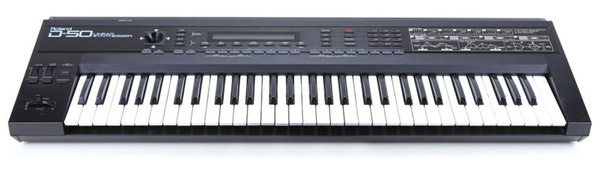
\includegraphics[width=.85\textwidth]{Images/roland_d50.jpg}
\caption{Roland D-50}
\label{fig:fullfig}
\end{figure}

\textbf{Quick Patching}
\begin{enumerate}
	\item Select the bank number with the numbers on the lower left side
	\item Select the patch number within the ban with the numbers on the lower right side
	\item Press [PATCH EDIT] and select the parameters to change in the menu
	\item The Modulation Bender and [PORTAMENTO] on the left side allow for live changes
\end{enumerate}

\newpage
\subsection{Korg Triton Extreme}
The Korg Triton made its debut in 2004. It is a workstation and sampler (16 MB sample RAM, 2 minutes and 54 seconds in mono at 48 kHz), has a programmable arpeggiator, ribbon controller, 2 USB ports, and "Valve Force" which can convert the signal into analog form. Notable users are: David Bowie, Coldplay, Lady Gaga, Ronald Jenkees, Linkin Park, Moby, Paul Oakenfold, Scooter, Mike Shinoda, Serj Tankian, and Timbaland. \\
\linebreak
\href{https://github.com/dkadyrov/MIDILab/blob/master/Manuals/Korg_Triton_Extreme.pdf}{Korg Triton Extreme Manual (PDF)}

\begin{figure*}[h]
\centering
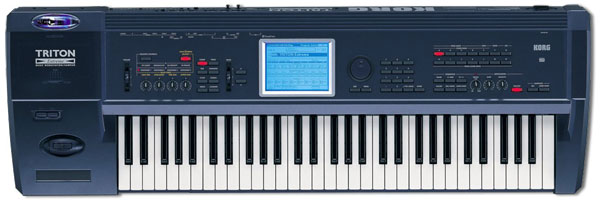
\includegraphics[width=.85\textwidth]{Images/tritonextreme.jpg}
\caption{Korg Triton Extreme}
\label{fig:fullfig}
\end{figure*}

\textbf{Edit Suggestions}
\begin{enumerate}
	\item Press [PROG] (Program) Mode
	\item Press Bank \& Program keys, turn dial, use touchscreen or use up and down keys to select patches.
	\item Press [MENU]
	\item Press [REAL TIME CONTROLS]
\end{enumerate}

\textbf{Add Effects}
\begin{enumerate}
	\item Press [MENU] key, Page Jump Menu, press P8 (or hold MENU key down)
	\item Press routing tab in window, choose IFX
	\item Press Insert FX tab at the bottom of the window and choose a tab at the bottom of the window
	\item Choose desired effect (change to ON by pressing OFF button)
	\item Check CHAIN box to add another effect; press OFF button of that effect to change to ON
\end{enumerate}

\newpage

\newpage

\subsection{E-mu Proteus 2000}

	The E-mu Proteus 2000 was released in 1999. Contains thousands of waves utilizing 32 MB of ROM. Features 128 voice polyphony and 32-part multi-timbrality. E-mu Systems became a popular company with their Emulator sampler and continued to pioneer sample-based synthesis with the Proteus range. The sampler does not allow users to record sounds, but offers a range of factory sounds that then can be layered, filtered, modulated by LFO's, and shaped by envelopes. \\
\linebreak
\href{https://github.com/dkadyrov/MIDILab/blob/master/Manuals/EMU_Proteus2000.pdf}{E-mu Proteus 2000 Manual (PDF)}


\begin{figure*}[h]
\centering
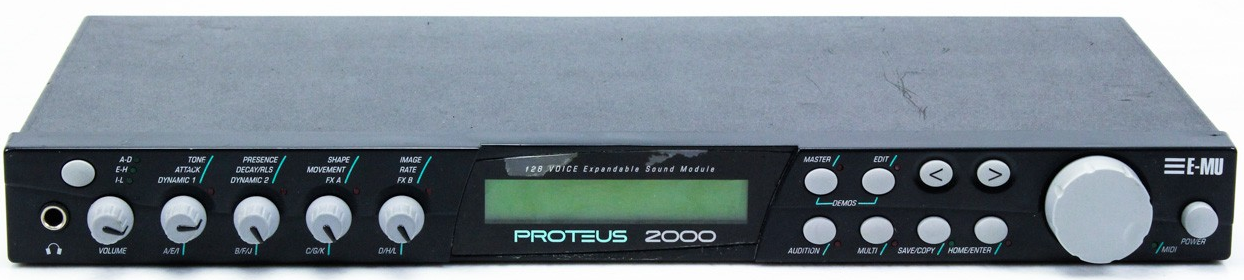
\includegraphics[width=.85\textwidth]{Images/e-mu-proteus-2000}
\caption{E-mu Proteus 2000}
\label{fig:fullfig}
\end{figure*}

\textbf{Quick Patching}
\begin{enumerate}
	\item Turn the large knob (data entry knob) to switch through patches
	\item Change parameters with the 5 smaller knobs (realtime control knobs) on the left side. The button to the left of the realtime control knobs changes the function of the row of knobs (written list above knobs).
	\item For more complex control, press the [EDIT] button and use the data entry knob to select the parameters you want to change. Press the in the data entry knob as an enter function and then change the data values by turning the knob.
\end{enumerate}

\newpage

\newpage
\section{Audio Equipment}
\subsection{Audio Signal Path}

\begin{figure*}[h]
\centering
\includegraphics[width=.85\textwidth]{Images/BlockDiagramAudio.png}
\caption{Block Diagram of Audio Signal Path}
\label{fig:fullfig}
\end{figure*}

\subsection{Line 6 TonePort MK2}

The audio interface for the MIDI Lab. Please do not change any parameters on the hardware or the supporting software. The TonePort is really advertised for use with a guitar, if you would like to record one feel free to plug it into the $\frac{1}{4}$" port of audio interface.

\subsection{DMV-Pro Effects Processor}

The DMV-Pro is the MIDI Lab's hardware effects processor with dual true-stereo inserts. To send audio to the effects processor, select the synth channel and pot the first two red auxiliary knobs. To change the parameters, rotate the three large black knobs on the effects processor.\\
\linebreak
\href{https://github.com/dkadyrov/MIDILab/blob/master/Manuals/DMV_Pro.pdf}{DMV-Pro Effects Processor Manual (PDF)}

\begin{figure*}[h]
\centering
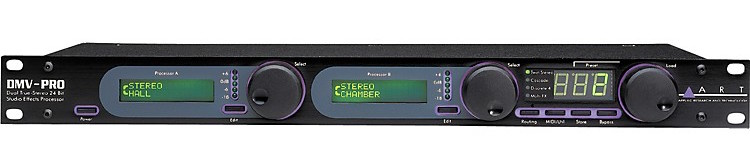
\includegraphics[width=.85\textwidth]{Images/DMVPRO.jpg}
\caption{DMV-PRO Effects Processor}
\label{fig:fullfig}
\end{figure*}

\newpage
\subsection{Mackie CR1604 VLZ Mixer}

16 channel audio mixer with ability to send audio to effects processor, other keyboards (for sampling), and for recording on the iMac as well as to a personal computer through a personal audio interface.\\
\linebreak
\href{https://github.com/dkadyrov/MIDILab/blob/master/Manuals/Mackie_Manual.pdf}{Mackie CR1604 VLZ Mixer Manual (PDF)}


\begin{figure}[h]
\centering
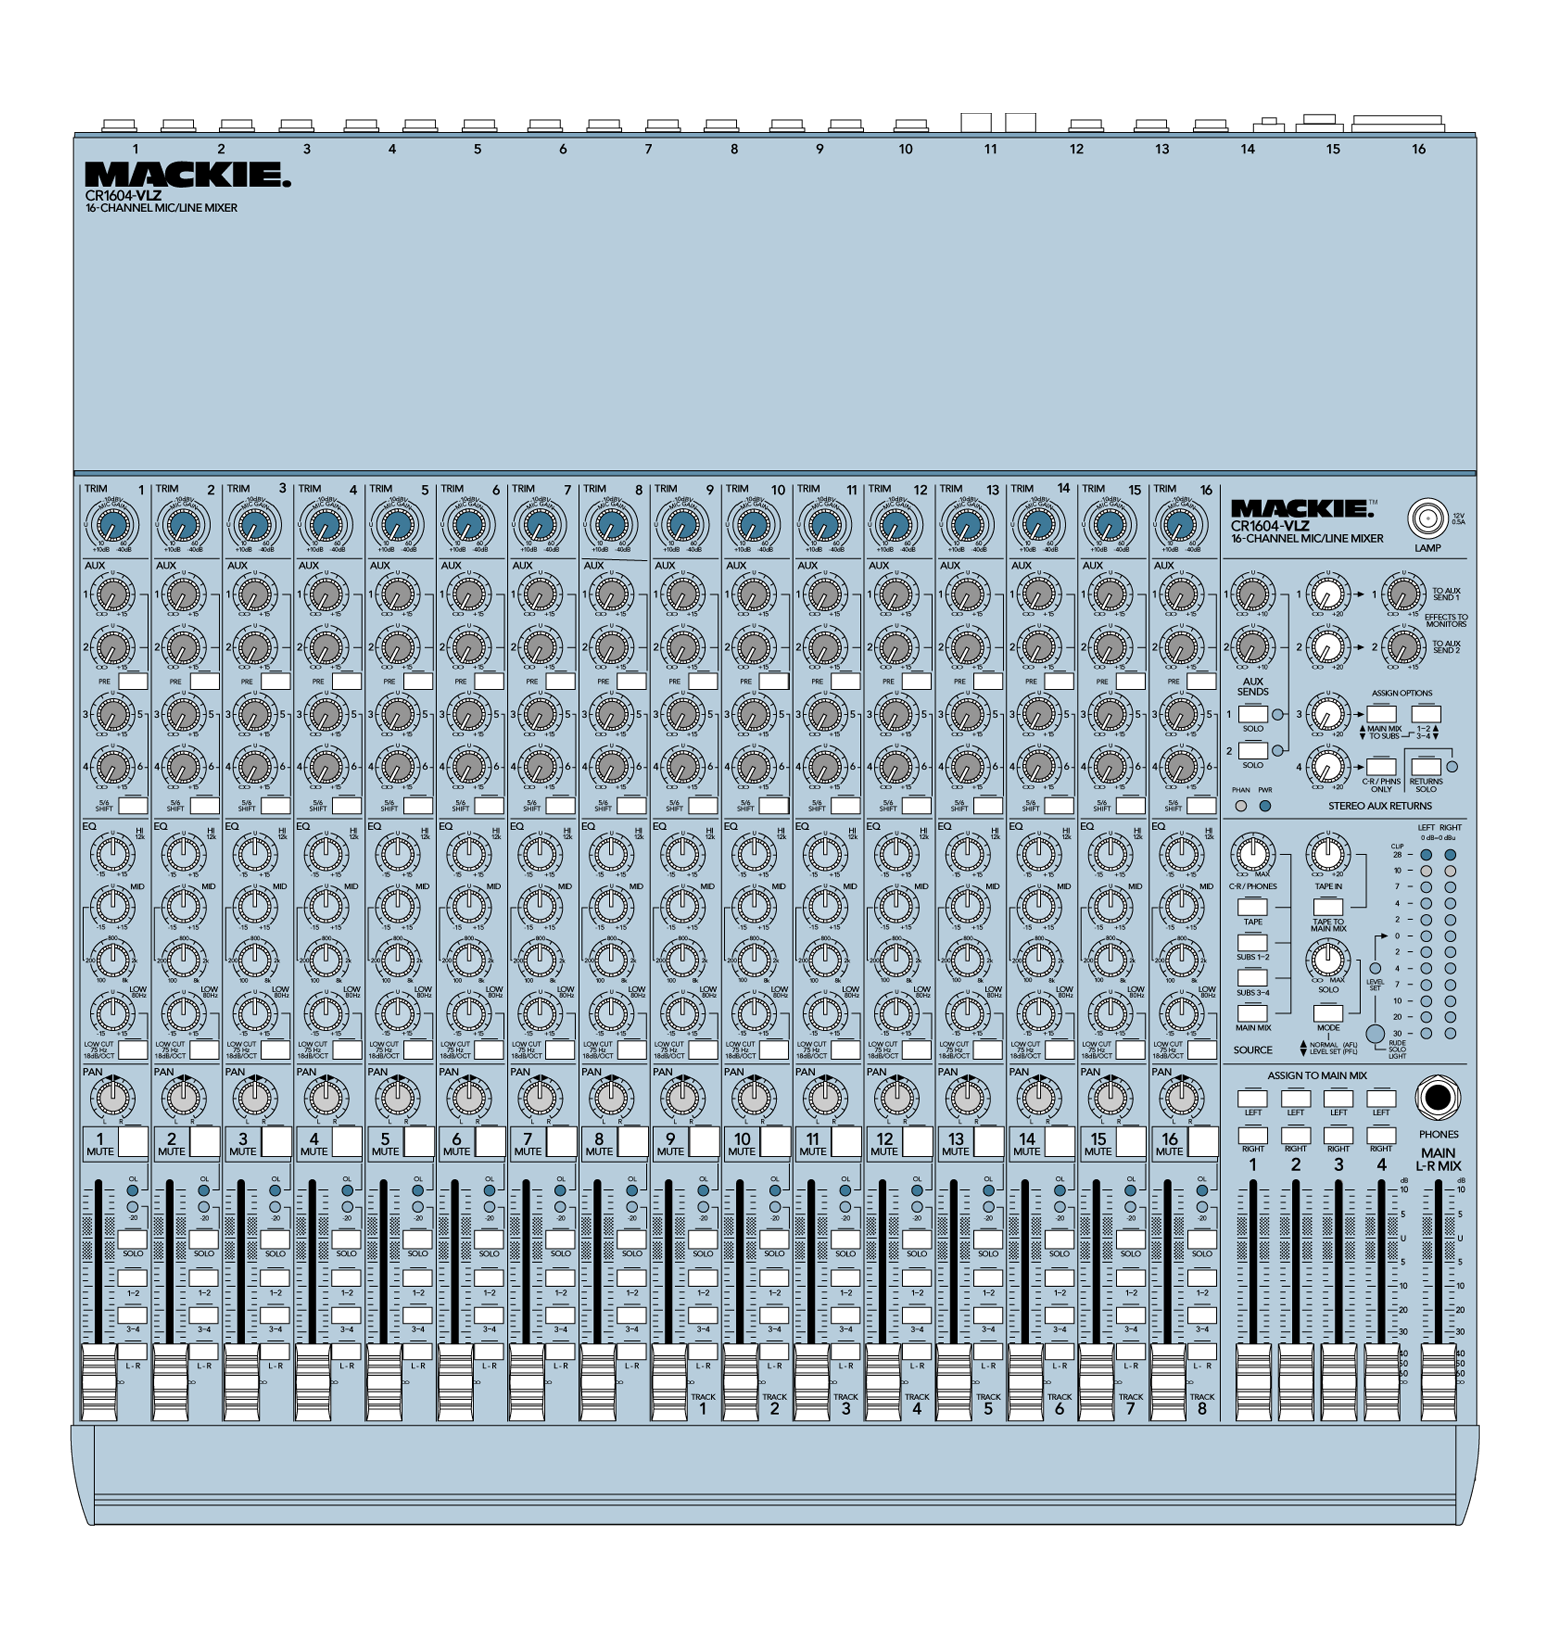
\includegraphics[width=.85\textwidth]{Images/Mackie_Manual-1.png}
\caption{Mackie CR1604 Mixer}
\end{figure}

\newpage

\subsubsection{Control of Individual Channel}

\begin{multicols}{2}
\small
\begin{enumerate}
	\item Volume Fader: Controls the volume of the channel within the mixer
	\item Path (Subs): Chooses where the channel signal is directed to
	\begin{enumerate}
		\item \textbf{Solo}: Isolates the channel in the mix. Useful for when you only want to hear the specific channel without other ones.
		\item \textbf{1-2}: Sends to Computer for Recording
		\item \textbf{3-4}: Sends to stereo $\frac{1}{4}$" cables for use with personal audio interfaces.
		\item \textbf{L-R}: Sends only to Monitors (Speakers)
	\end{enumerate}
	\item Mute: Mutes the Channel
	\item Pan: Controls the amount of signal sent to the left vs right, 1 vs 2, or 3 vs 4
	\item Equalization (EQ)
	\begin{enumerate}
		\item \textbf{High EQ}: $\pm 15$ dB at $12$ kHz
		\item \textbf{Mid EQ}: $\pm 15$ dB within 1.5 octaves of the frequency center (Determined by Frequency Sweep)
		\item \textbf{Frequency Sweep}: Selects the center of the Mid EQ between $100$ Hz and $8$ kHz
		%\item \textbf{Low EQ}: $\pm 15$ dB at $80$ Hz
		\item \textbf{Low Cut Switch}: Removes all signal below $75$ Hz (High Pass Filter)
	\end{enumerate}
	\item Auxiliary Sends: Sends a parallel signal path to other outputs on the mixer. See \ref{fig:signal} for more information.
	\begin{enumerate}
		\item \textbf{Aux A-B}: The DMV Pro effects processor has two inputs and can run different effects on each input. Aux \textbf{A} sends a signal to input 1 on the processor and Aux \textbf{B} sends a signal to input 2. See the section on the \hyperlink{effects processor}{effects processor}.
		\item \textbf{Aux C-D}: Not used
	\end{enumerate}
	\item Trim (Gain): Controls the amplitude of the signal going into the mixer. Input sensitivity is adjusted by $-10$ dB to $40$ dB. Please do not adjust unless necessary.
\end{enumerate}

\begin{center}
  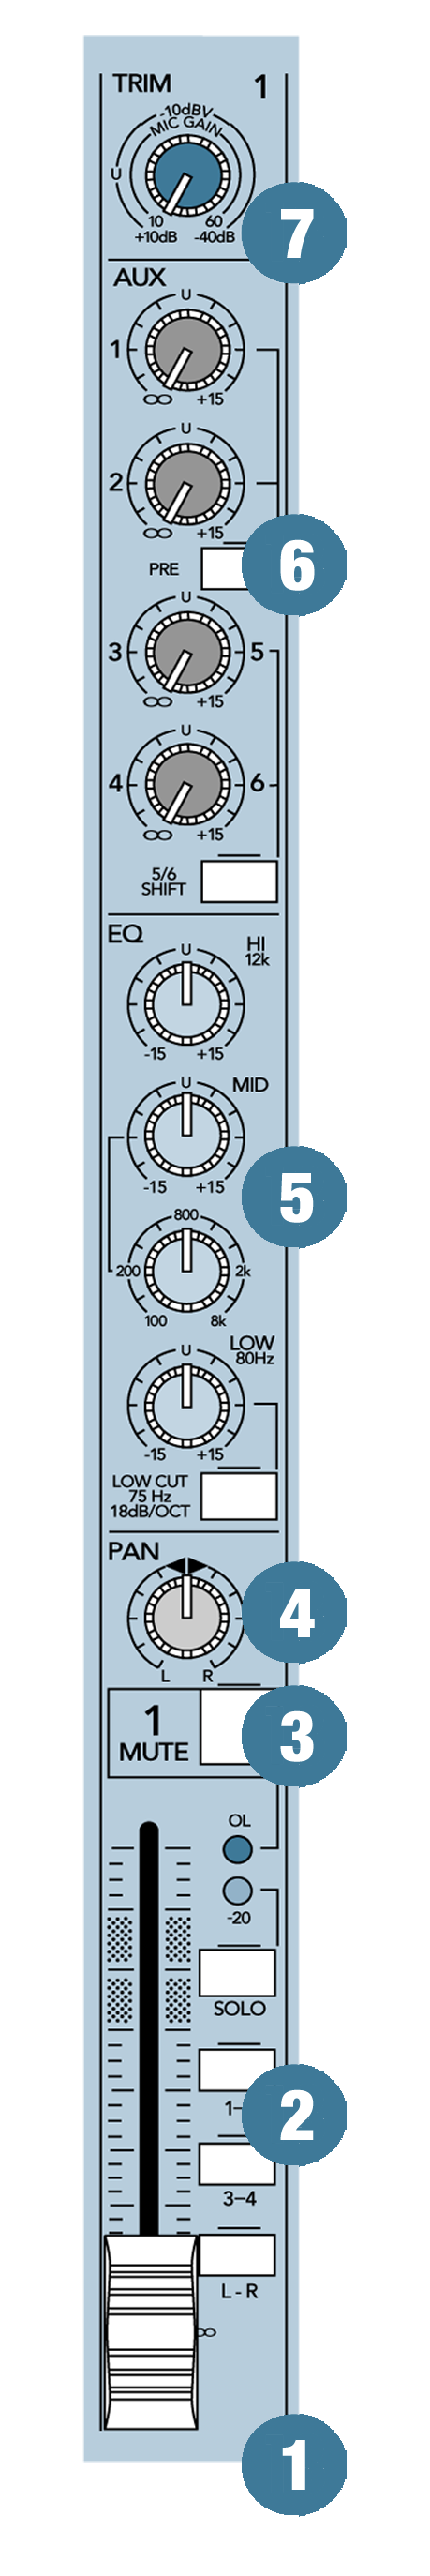
\includegraphics[height=220mm]{Images/Mackie.png}
  %\captionof{figure}{AA \cite{BB}}
\end{center}

\end{multicols}

\newpage

\subsubsection{Control of Mixer}
\begin{multicols}{2}
\small
\begin{enumerate}
	\item Effects to Monitors: Adds effects to monitors.
	\item Aux 1-2 Sends: Controls the gain of the AUX 1-2 send output into the mixer.
	\item AUX Returns: Controls the volume of the signal returning from the AUX within the mixer.
	\item 1-2/3-4 Toggles: Controls the path of the signal to
	\item IGNORE ABOVE
	\item C-R/Phones: Controls volume to the Control Room out and the Headphone Jack
	\item Selects what inputs are routed to the meter display
	\item Meter Display: Visually shows the strength of the signal. Want the highest possible signal strength (green) without clipping (red light). At yellow compression occurs.
	\item Selects what inputs are routed to the meter display, the C-R out and the headphone jack.
	\item Solo Knob: Controls the level of the soloed channels
	\item Mode Control:
	\begin{enumerate}
		\item \textbf{Normal (AFL)}: solo signal is post EQ, Pan, and Fader
		\item \textbf{Level Set (PFL)}: solo signal is pre EQ, Pan, and Fader
	\end{enumerate}
	\item \hypertarget{Headphone Jack}{Headphone Jack}: Accepts $\frac{1}{4}$ in. plug. Feel free to use your own headphones.
	\item Main Mix Assigns: Allows fader subgroups 1-4 to be assigned left, right, or both channels in main mix.
	\item Subgroup Volume Faders: Control the output levels of chosen group. Adjusting the volume of subgroup 1-2 will change the volume audio into the iMac. Adjusting 3-4 will change volume of the audio going into personal audio equipment.
	\item Master Fader: controls output to speakers.
\end{enumerate}
\begin{center}
  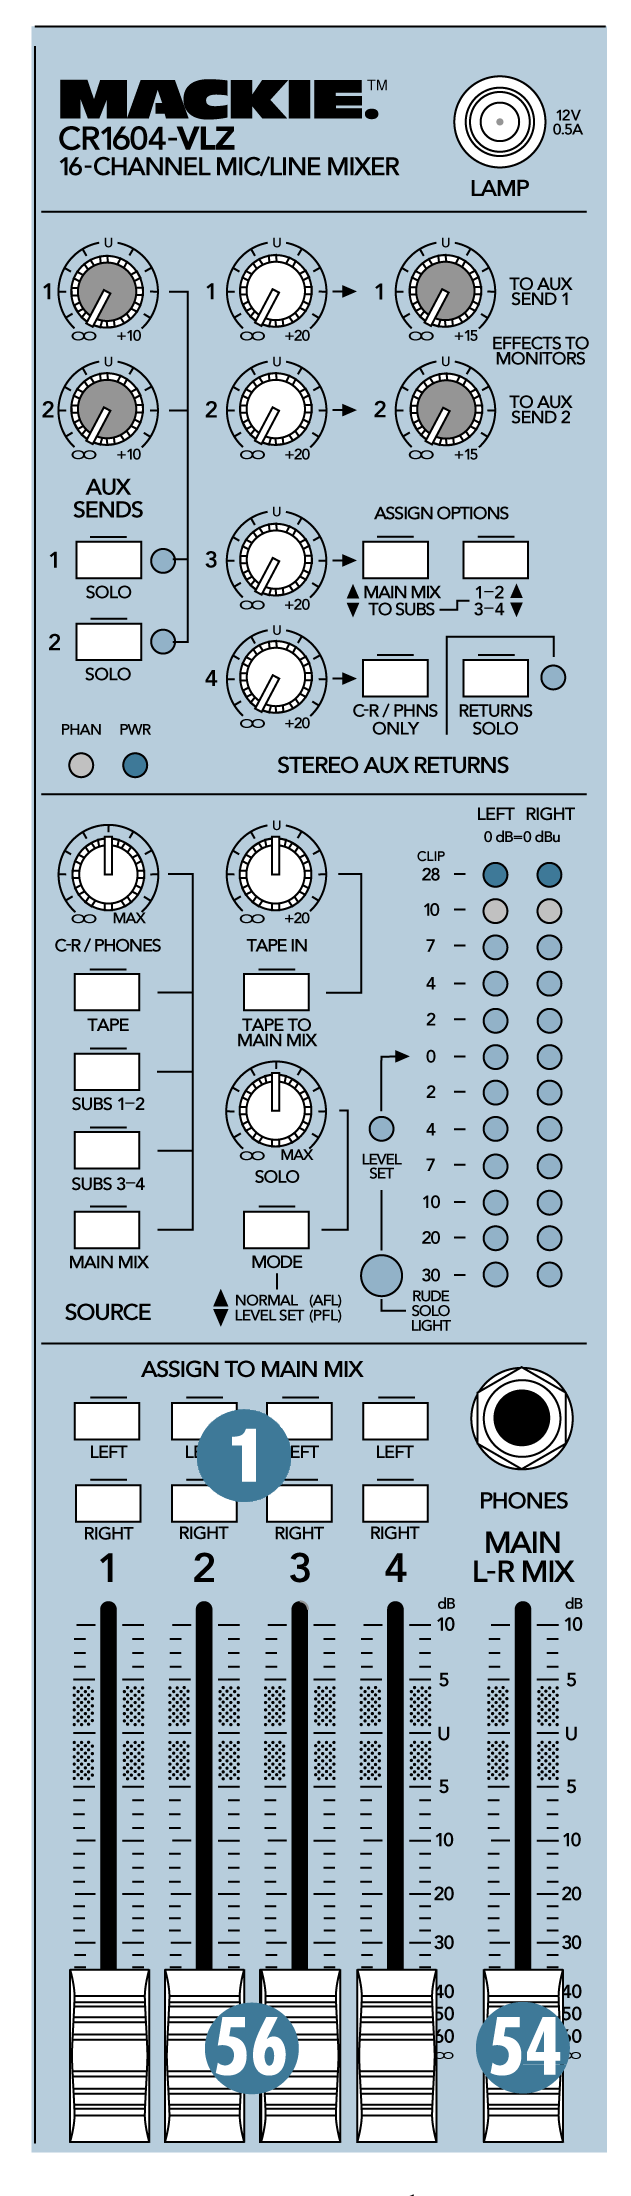
\includegraphics[height=220mm]{Images/Mackie_2.png}
  %\captionof{figure}{AA \cite{BB}}
\end{center}
\end{multicols}




\newpage
\newpage
\section{MIDI Equipment}
\subsection{MIDI Signal Path}

\begin{figure*}[h]
\centering
\includegraphics[width=.85\textwidth]{Images/BlockDiagramMIDI.png}
\caption{Block Diagram of MIDI Signal Path}
\label{fig:fullfig}
\end{figure*}

\subsection{Yamaha Clavinova CLP-50}

The Yamaha Clavinova CLP-50 is used as the MIDI controller in the MIDI Lab. It is used to control the other synthesizers and the DAW. By default the keyboard plays sound through its built in speaker. To turn this off, turn local off. \\

\textbf{To Turn Local Off} 

\begin{enumerate}
	\item Press and hold [TRANSPOSER]
	\item While holding [TRANSPOSER], press [PIANO NORMAL]	
\end{enumerate}

\newpage

\subsection{MOTU MIDI Time Piece MTP AV}
The Mark of the Unicorn MIDI Time Piece allows for MIDI communication between the MIDI controller (Yamaha Clavinova), the iMac, and the other synthesizers in the MIDI lab. \\

\begin{figure*}[h]
\centering

\includegraphics[width=.85\textwidth]{Images/MOTU.jpg}
\caption{MOTU MIDI Time Piece MTP AV}
\label{fig:fullfig}
\end{figure*}

\textbf{Control other synths using Yamaha Clavinova}
\begin{enumerate}
	\item Turn the [VALUE] knob until desired synth is selected (Computer, Korg Triton, Roland D-50,  E-mu Proteus 2000)
	\item Select the synth using the [YES/NO ENTER] button
\end{enumerate}

\textbf{Send MIDI from DAW to Synth}
\begin{enumerate}
	\item In chosen DAW create a MIDI channel 
	\item Have the MIDI To send to "MIDI Timepiece Port 1" for the Korg Triton, "MIDI Time Piece Port 2" for the Roland D-50, and "MIDI Time Piece Port 3" for the E-mu Proteus 2000. 
\end{enumerate}
\end{document}

